% This is samplepaper.tex, a sample chapter demonstrating the
% LLNCS macro package for Springer Computer Science proceedings;
% Version 2.21 of 2022/01/12
%
\documentclass[runningheads]{llncs}
%

\usepackage{graphicx}
\usepackage{amsmath}
\usepackage{amssymb}
\usepackage{booktabs}
\usepackage{amsmath}
\usepackage{commath}
\usepackage{tabularx}
\usepackage{url}
\usepackage{xspace}
\usepackage{algorithmic}
\usepackage{subfloat}
\usepackage{subcaption}
\usepackage{bm}

%\usepackage[floatsintext]{float}
%\usepackage[caption=false]{subfig}
%\usepackage{subcaption}

\DeclareUnicodeCharacter{2212}{-}

%\newcommand\norm[1]{\left\lVert#1\right\rVert}
%\newcommand{\vectornorm}[1]{\left|\left|#1\right|\right|}
\newcommand{\argmin}{\operatornamewithlimits{argmin}}
\newcommand{\argmax}{\operatornamewithlimits{argmax}}
%\newcommand{\drdiff}{DrDiffGAT\xspace}
\newcommand{\drdiff}{DrGAT\xspace}

\usepackage[T1]{fontenc}
% T1 fonts will be used to generate the final print and online PDFs,
% so please use T1 fonts in your manuscript whenever possible.
% Other font encondings may result in incorrect characters.
%
\usepackage{graphicx}
% Used for displaying a sample figure. If possible, figure files should
% be included in EPS format.
%
% If you use the hyperref package, please uncomment the following two lines
% to display URLs in blue roman font according to Springer's eBook style:
%\usepackage{color}
%\renewcommand\UrlFont{\color{blue}\rmfamily}
%\urlstyle{rm}
%
\begin{document}
%
\title{Drug Response Prediction Through Controllable Diffusion and Graph Attention Network}
%
%\titlerunning{Abbreviated paper title}
% If the paper title is too long for the running head, you can set
% an abbreviated paper title here
%
\author{Emre Sefer\inst{1}\orcidID{0000-0002-9186-0270}}
%
\authorrunning{Sefer et al.}
% First names are abbreviated in the running head.
% If there are more than two authors, 'et al.' is used.
%
\institute{Ozyegin University, Istanbul, Turkey
\email{emre.sefer@ozyegin.edu.tr}}
%
\maketitle              % typeset the header of the contribution
%
\begin{abstract}

Accurately predicting drug responses based on a patient's genomic
profile is critical for advancing precision medicine. The rise of deep
learning algorithms leveraging large-scale omics datasets has been a key driver of research in this area. However, biological datasets,
which are typically high-dimensional but have small sample sizes,
present challenges such as overfitting and poor generalization in
predictive models. Complicating matters further, gene expression data must capture complex inter-gene relationships, exacerbating these issues. To tackle these challenges, we introduce a drug response
prediction framework, called \drdiff, which combines a denoising diffusion probabilistic model (DDPM) for data augmentation with a graph attention network-based prediction module. Our approach achieved a $10\%$ improvement in AUC compared to state-of-the-art models for the six drugs studied, indicating \drdiff's superior generalization capabilities. Moreover, our experiments confirm the potential of generative models, a core component of our framework, to mitigate the inherent limitations of omics datasets by effectively augmenting gene expression data.
%Our code and datasets can be found at~\url{https://github.com/seferlab/drdiff}.


%\keywords{First keyword  \and Second keyword \and Another keyword.}
\end{abstract}
%
%
%

\section{Introduction}

Precision oncology, which aims to provide personalized cancer
treatments based on the genetic characteristics of individual tumors,
avoids ineffective treatments, emerging as a promising approach for
improving patient outcomes and reducing healthcare costs~\cite{1}. This
could be leveraged toward the advancement of web-based precision
medicine, in light of the escalating availability of individual
medical data~\cite{21}. Accurately predicting drug responses, which
indicates how a specific drug is effective as a treatment, is greatly
becoming important in the current precision oncology. However,
variabilities in drug responses among patients, which are attributed to genetic variations, make obtaining accurate predictions
challenging~\cite{2}. Many studies have been conducted on deep learning
(DL) models that learn the genetic information of patients for drug
response predictions, with many previous studies~\cite{3, 4} revealing that
Gene Expression~(GE) data, which represents the measurement of the
activity of genes is the most effective type of data for drug
response predictions~\cite{6, 8, 22, 25}.

In bioinformatics, such as cancer subtype or drug response
prediction studies using omics data including gene expression data, high dimension
and low sample size of input data are fundamental challenges. Many
features or variables with relatively few input data samples increase
the risk of overfitting in training datasets and reduce the generality
of prediction models~\cite{1, 23, 24}. Additionally, the robustness of
such models is affected by outliers in datasets with small sample
sizes. Therefore, it is essential to carefully balance the number of
features and sample sizes when conducting data analysis, particularly
for omics data, which are often characterized by large dimensions and
small sample sizes. In this study, we aim to overcome these obstacles.

To effectively address the aforementioned problem, approaches from
various perspectives have been proposed: Feature Selection, Data
Augmentation, Utilizing Inductive Bias. The strategy from the feature
selection perspective is to select only genes closely related to the
drug or disease by utilizing biological pathways~\cite{9, 14}. The
experimental results in these studies revealed that feature selection
using biological pathways would be an appropriate approach to reduce
high dimensionality. A second possible solution would be to augment
training data by utilizing generative models, such as variational
autoencoders~(VAEs)~\cite{4} and generative adversarial networks~(GANs)~\cite{19}, which have been actively studied in the field of image
processing. Notably, there is a study that proposes improvements in
cancer classification performance by augmenting GE data using a GAN
and one that proposes a universal tabular generative model that can be
applied to data such as gene expression data~\cite{5, 35}. However, these studies do not
account for generative models neglecting to consider the relationship
between genes when learning, which limits their ability to capture
biological mechanisms. Additionally, the advancement in the field of
generative models have led to the emergence of innovative models such
as DDPM~\cite{17, 32}, which exceeds the capabilities of GAN and VAE. These models present new possibilities for utilization in augmentation tasks, which aim to alleviate data sparsity. Lastly, to overcome the degradation of model predictive power due to limited training data, a strategy is to use the relationships between genes as an inductive bias for the predictive model~\cite{3, 15}. This approach can
be realized by utilizing graph neural networks that can learn the
relationships between biological pathways obtainable from various
databases~\cite{20}. However, to increase the predictive power
more efficiently with limited data, there is a need for approaches
that not only efficiently integrate multiple biological pathways but
also better capture biological mechanisms by training models to
identify the importance of relationships between genes in predicting
drug responsiveness.

To overcome the limitations of existing studies, we propose a framework capable of addressing the overfitting problem in training data caused by the high dimensionality and low sample sizes in omics datasets in the context of drug response prediction. The proposed framework \drdiff comprises three main modules: 1- Feature selection
through biological pathway analysis to solve the issue of high
dimensionality, 2- Gene expression data augmentation utilizing diffusion-based
generative models~(Diffusion-GE) to address the issue of low sample
sizes, and 3- Drug response prediction using graph attention
networks. The first module aims to solve the problem of high
dimensionality by extracting the biological pathways most closely
related to the target protein of each drug and selecting the genes
that comprise these pathways. The second module aims to augment GE
data by leveraging a recent generative model~(Denoising Diffusion
Probabilistic Model), in which a graph autoencoder~(AE) is employed
to capture biological mechanisms. The final module employs a graph
attention network, which exploits prior knowledge about biological
pathways to maximize the generalization of models from limited
training data.

The main contributions of the study are summarized as follows:
%
\begin{itemize}
\item To the best of our knowledge, this is the first study to adapt and enhance the recently developed Denoising Diffusion Probabilistic Model~(DDPM) for developing a GE data augmentation model that captures biological complexities and addresses the issue of omics~(gene expression) data scarcity.
\item We present a novel approach for highly accurate drug response prediction. Our approach leverages the capabilities of a graph attention network, which effectively combines information from a wide range of biological pathways while also considering the proximity to target proteins.
\item The proposed framework, \drdiff, demonstrated superior performance in drug response prediction on patient datasets not seen during training, surpassing other recent methods. Furthermore, we presented evidence of the generative module, a core component of our framework, consistently generating higher-quality data compared to data produced by other generative models.
\end{itemize}
    
\section{Related Work}

Numerous approaches have been used for drug response predictions. Traditionally, machine learning techniques have been utilized to select crucial features for prediction~\cite{8, 11, 13, 18}, and AEs have been employed for feature extraction to enhance the prediction performances of models~\cite{36}. In recent years, with the advancement of various DL techniques, research on drug response predictions has evolved. One such model, Multi-Omics Late Integration~(MOLI)~\cite{29}, utilizes a deep neural network architecture that enables the integration of multiple omics data types at different stages of a network. Supervised feature extraction learning using triplet loss~(Super.FELT)~\cite{25}, on the other hand, employs feature selection to reduce the dimensionality of multi-omics data, followed by a supervised encoder that extracts crucial information from the reduced omics dataset. Then, it classifies the encoded omics datasets based on a neural network for drug response prediction. A novel model, DeepInsight-3D~\cite{30}, converts structured data into images using convolutional neural networks~(CNNs) for predicting patient-specific anticancer drug responses.


\section{Preliminaries}

A set of biological pathways, denoted as $G = \{G_1, G_2, \ldots,
G_k\}$, is defined on a set of subgraphs $G=(V, E)$. Subgraph $G$ denotes
an undirected graph comprised of a set of nodes $v_i \in V$ and a set
of edges $e_i = (v_i, v_j) \in \mathcal{E}$. Each node represents a gene, and an edge represents a relationship between genes.

\subsection{DDPM}

A Denoising Diffusion Probabilistic Model~(DDPM)~\cite{17} is designed to
learn a Markov Chain that systematically transforms a basic probability distribution, often a random Gaussian distribution, into a distribution that resembles actual data. This generative process is essentially the reverse of the forward diffusion process within DDPM. In this forward process, a fixed Markov chain progressively introduces noise to data while sequentially sampling latent variables $x_0, x_1, \ldots, x_T$, all having the same dimensionality. Each step in the forward process is a Gaussian translation.
%
\begin{equation}\label{eq:1}
q(x_t | x_{t-1}) := N(x_t; \sqrt{1-B_t} x_{t-1}, B_{t}\bf{I})
\end{equation}
%
where $\beta_1, \beta_2, ldots, \beta_T$ are predetermined variance settings rather than parameters that the model learns. Eq.~\eqref{eq:1} calculates $x_T$ by introducing minor Gaussian noise to the latent variable. Given clean data $x_0$, the sampling of $x_T$ is expressed in a closed form by reparameterization trick as follows:
%
\begin{align}
 & q(x_t | x_{0}) = N(x_t; \sqrt{\overline{a}_t} x_0, (1-\overline{a}_t) \bf{I}) \label{eq:2} \\
& x_t = \sqrt{\overline{a}_t} x_0 + \sqrt{1-\overline{a}_t} \epsilon \label{eq:3}
\end{align}
%
where $\alpha_t := 1-\beta_t$, $\overline{\alpha}_t := \prod_{s=1}^{t} \alpha_s$, and $\epsilon \sim N(0, \bf{I})$ is a random Gaussian distribution with the same dimensionality as $x_0$.

The training strategy of DDPM commences with the parameterization $p_{\theta}(x_{t-1} | x_t)$ of Gaussian transitions in the reverse direction of the forward process, which injects noise. Subsequently, the strategy culminates in training the reverse process's mean to predict the mean of the forward process to learn the reverse process's transition kernel.
%
\begin{align}
p_{\theta}(x_{t-1} | x_t) = N(x_{t-1};   \mu_{\theta}(x_t, t),
  \sigma_{t}^2 \bf{I}) \label{eq:4} \\
L_{\text{simple}} :=  \mathbb{E}_{t, \epsilon, x_0} \left[ || \epsilon - \epsilon_{\theta} (\sqrt{\overline{a}_t} x_0 +
  \sqrt{1-\overline{a}_t} \epsilon, t) ||^2 \right] \label{eq:5}
\end{align}

Eq.~\eqref{eq:2} provides an efficient method to jump directly to an
arbitrary step in the forward noise process, making it possible to
randomly sample $t$ during training. To predict $\mu_{\theta}(x_t, t)$
efficiently,~\cite{17} adopted a specific parameterization
approach based on Eq.~\eqref{eq:4}-\eqref{eq:5}. Hence, a trainable neural
network could predict the noise added to $x_0$. These authors found that
using $\epsilon$ in prediction produced the best results, especially
when it was combined with a reweighted loss function as in Eq.~\eqref{eq:5}.


\section{Framework Design}

In this section, we introduce the proposed \drdiff framework for drug response prediction. Figure~\ref{fig:1} illustrates the overall process of the proposed framework.

\subsection{Network Analysis for Feature Selection}\label{sec:network}

To identify the biological pathways that most significantly impact drug response prediction results, the proximal pathways that are statistically associated with drug-associated genes need to be identified. We calculated the proximal pathway by measuring the distance from the drug-associated genes to each pathway as seen in Figure~\ref{fig:1}A, by using the method proposed in~\cite{14}. The measurement was based on the average shortest path lengths between the drug-associated genes and the nearest pathway genes, according to:
%
\begin{equation}
d_{\text{closest}} = \frac{1}{|T|} \sum_{t \in T} \min_{s \in S} d(s,t)
\end{equation}
%
where $T$ represents the set of drug-associated genes~(target genes), $S$ represents the pathway genes, and $d(s, t)$ is the shortest path
between the drug-associated and pathway genes. 

To identify whether the calculated distance for each pathway was statistically significant regardless of the number of nodes~(genes) that made up the pathway, random genes were bootstrapped to generate a reference distribution. We randomly selected genes by matching the size and number of the network neighbors~(degree) of the original drug-associated genes and pathway genes and computed the closest distance. The mean and standard deviation of the reference distribution were used to calculate the $z$-scores. When the $z$-scores for each pathway were sorted in ascending order, the top $K$ pathways were considered proximal. Finally, among all the genes, those that
most significantly impacted drug response predictions, namely those
included in the selected pathways, were selected for further analysis.

% \begin{figure}[!h]
% \centering
% 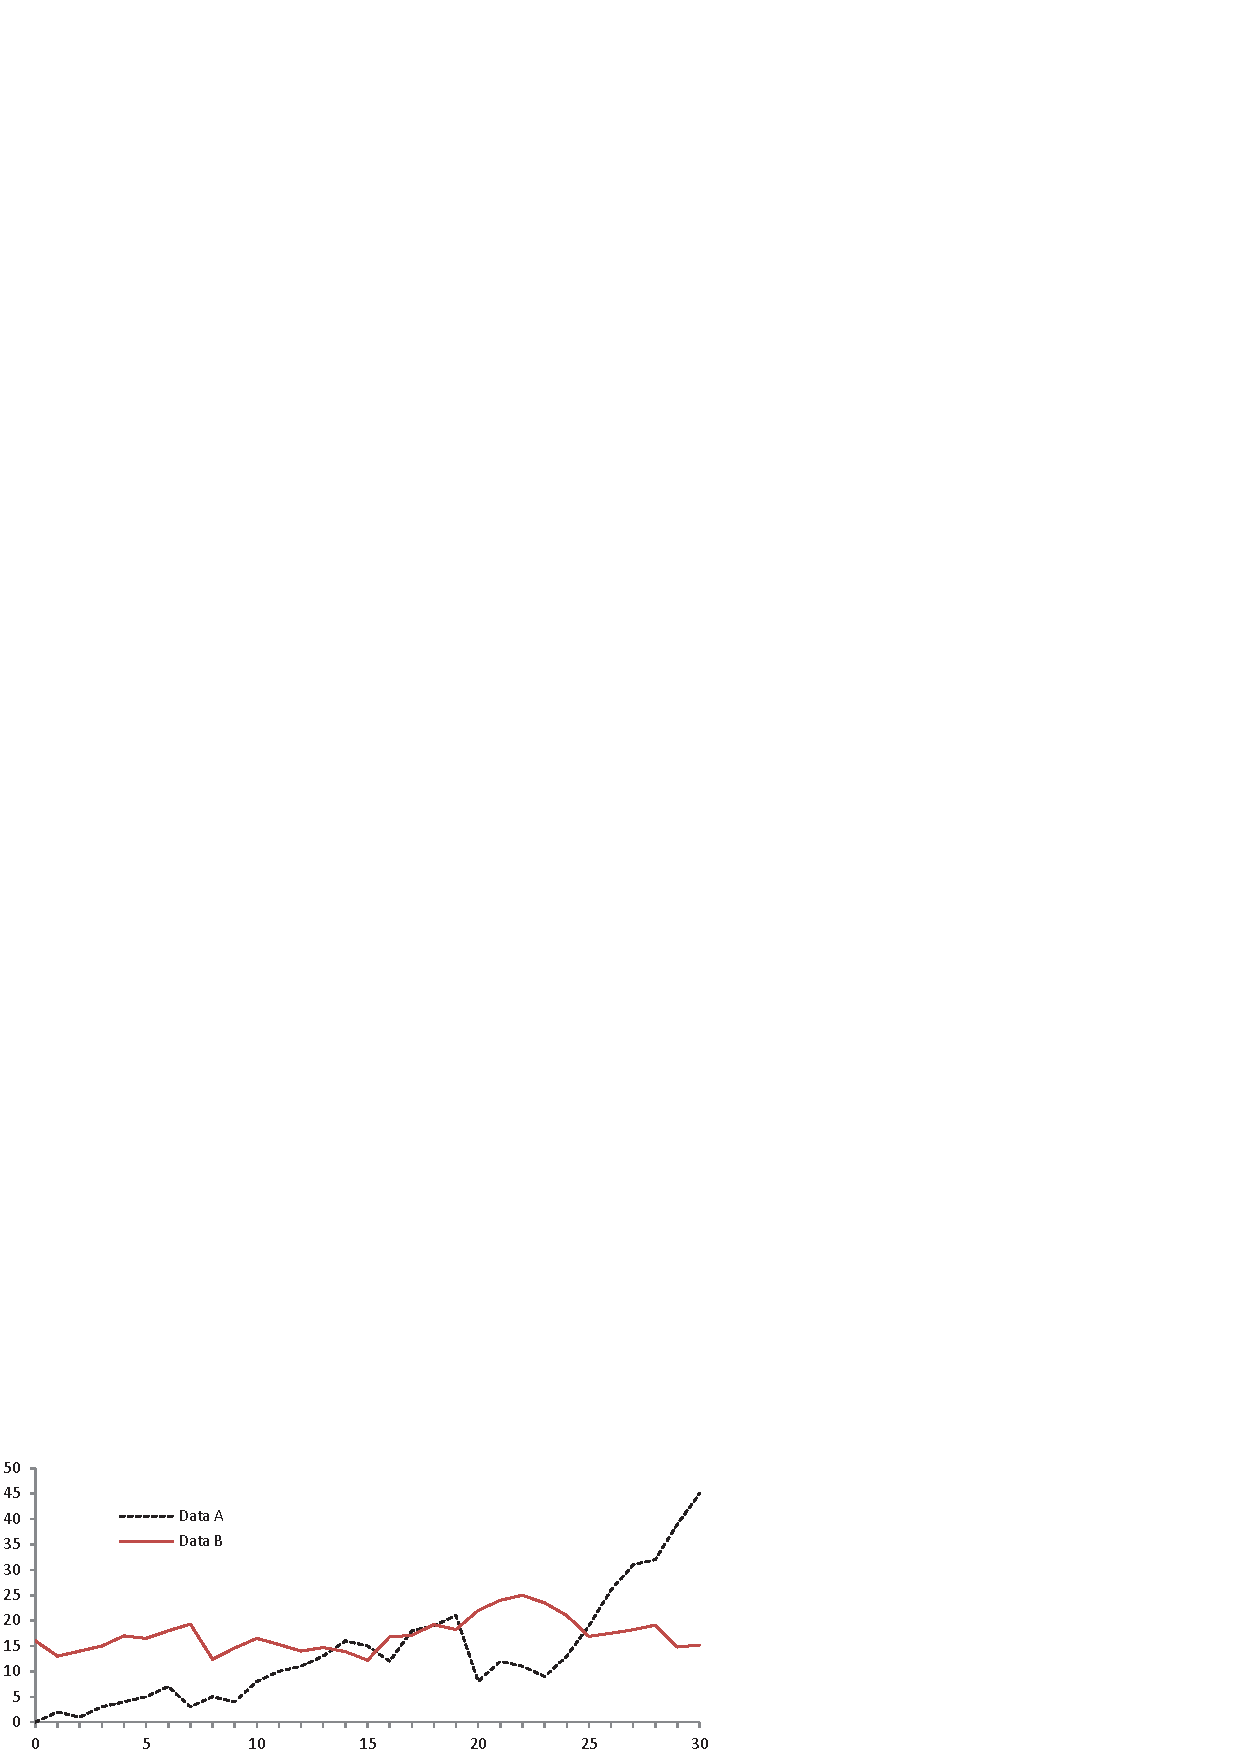
\includegraphics[width=0.99\textwidth]{fig1.png}
% \caption{Overview of the proposed \drdiff framework.}
% \label{fig:1}
% \end{figure}

\subsection{Data Augmentation and Generalization}\label{sec:augment}

This subsection introduces the second module of the proposed framework, a novel data augmentation method that addresses the lack of generalization due to insufficient training data as seen in Figure~\ref{fig:1}B. The module comprises two main components. The first component leverages the graph AE to map gene expression data to the latent space. The second component generates the latent space obtained using the DDPM. Finally, the augmented latent space is converted back to the gene expression data level using the trained decoder of the graph AE as seen in Algorithm~\ref{alg:1}.

\subsubsection{Graphical Compression of Gene Expression Profiles}\label{sec:compress}

The proposed graphical compression model was based on the AE architecture. It took the network information of the biological pathways representing the top $K$ pathways proximal to the target protein extracted through the method described in section~\ref{sec:network} as an input and encoded this into a graph representation latent space. The gene expression data $X \in R^{N \times d}$ input to the AE model represented each biological pathway~(extracted in Section~\ref{sec:network}) as one subgraph, as shown in section~\ref{sec:gat}, where the node features of the subgraph comprised gene expression profiles and gene indicators. Likewise, the encoder layer is defined with the same architecture as the graph attention layer used in Section~\ref{sec:gat}, and the affine layer was added to produce latent representations $X \in R^{N \times d} (d << D)$ of the input data after the graph attention operation. Subsequently, a decoder comprising affine layers was trained to reconstruct the initial node state, which contained only the gene expression profiles. Training was
done by optimizing the $L_{\text{graphAE}}$ loss function with respect to $\phi$ and $\psi$ as follows:
%
\begin{equation}
L_{\text{GraphAE}} = \sum_{i=1}^{N} (x_i - De_{\phi}(En_{\psi}(x_i, G)))^2
\end{equation}

Subsequently, the generative model introduced in the next section is designed to generate the latent space extracted in this section.

\subsubsection{Generative Modeling of Latent Space}

Regarding the trained graph AE model, which comprised $En_{\psi}$ and $De_{\phi}$, it had access to a low-dimensional latent space containing information about biological relationships. Additionally, contrasting with the image generation task in which the DDPM is commonly used, in this study, this model required modifications to generate latent spaces containing gene expression information and the relationships between genes.

In the field of image generation, the backbone architecture of the
DDPM-based model is implemented as U-Net~\cite{unet} because CNN
operations that form the U-Net architecture align well with the
inductive bias of image-like data. However, in our case, adopting a
CNN-based U-Net model as a backbone architecture is inappropriate
because, unlike images, the data to be covered do not exhibit locality
or dependencies among neighboring pixels. Therefore, considering the
characteristics of the gene expression data, we updated the backbone architecture from a convolution layer to an affine layer.

The module discussed in this section enhances the predictive
performance of the model in determining the sensitivity or resistance
of a sample to a drug, by increasing the amount of training data. To
achieve this, instead of unconditionally generating samples, samples
with labeled indications of their sensitivities or resistances to
drugs should be generated. In the conditional generation setting, the
input data $x_0$ had an associated condition term~(sensitive group and
drug-resistant group). Then, the diffusion model needs to be modified to include condition term $c$ as an input to the reverse process for learning a conditioned generative model $p_{\theta}(x_0|c)$.
%
\begin{equation}
p_{\theta}(x_{t-1}|x_t) = N(x_{t-1}; \mu_{\theta}(x_t, t, c), \sigma_{t}^2\bf{I})
\end{equation}

The reverse process, in which denoising occurs, is transformed into a
conditional probability according to the given condition. Additionally, the
injection of noise is the same for data belonging to any class,
indicating that the forward process is not transformed based on the
condition or class of the data. When the mean in the reverse process
changes from $\mu_{\theta}(x_t, t)$ to $\mu_{\theta}(x_t, t, c)$, $c$ should be added as an extra input to the trainable backbone architecture function approximators. In this case, depending on the modification of the reverse process, the original simplified loss function as defined in Eq.~\eqref{eq:5} can be rewritten as follows:
%
\begin{equation}
L_{\text{cond}} :=  \mathbb{E}_{t, \epsilon, x_0} \left[ || \epsilon - \epsilon_{\theta} (\sqrt{\overline{a}_t} x_0 + \sqrt{1-\overline{a}_t} \epsilon, t, c) ||^2 \right]
\end{equation}

To sample latent variables that encompass biological information under specific conditions, it is necessary to adjust the stochastic generation step, which has been redefined as ancestral sampling by~\cite{17, 33}. The objective is to modify the inference process to generate stochastic samples that align with the specified conditions. This modification can be described as follows:
%
\begin{equation}
x_{t-1} = \frac{1}{\sqrt{\alpha_t}} \left( x_t - \frac{1-\alpha_t}{\sqrt{1-\overline{\alpha}_t}} \right) \epsilon_{\theta}(x_t, t, c) + \sigma_t z
\end{equation}
%
Finally, we performed decoding from the generated latent space to the gene expression data via a trained graph AE model.

Section~\ref{sec:response} describes the data augmentation method proposed for gene expression profiles to improve the generalization performance of drug response prediction models. This method aims to overcome the difficulty of generating gene expression data by using a compression~(Graph AE) model to map a low-dimensional latent space from GE data that captures biological structure information and then generates that latent space with the DDPM model; this method offers several advantages. By employing a graph AE to capture biological relationships during generative model training, the difficulty of model training is relatively reduced. Furthermore, mapping high-dimensional gene expression data to a low-dimensional latent space decreases computational complexity.

\subsection{Drug Response Prediction with Graph Network}\label{sec:response}

This section presents the final module of the proposed framework,
which is a drug-response prediction method that employs graph
attention networks as in Figure~\ref{fig:1}C. Specifically, each biological
pathway was represented as a subgraph $G=(V, E)$, and the graph
attention network model was applied to each subgraph to learn the
patterns of the gene relationships. Further details of this method
are provided below.

\subsubsection{Graph Attention Network}\label{sec:gat}

Each subgraph consisted of initial node features $X_i = H_{v_i}^{0} \in R^{N \times F}$ and edges $(v_i, v_j)$ describe the interaction between nodes. The node features comprised gene expression and indicators. Gene indicators were uniquely assigned to each gene using a trainable embedding matrix, resembling the process of token embedding in BERT~\cite{7}. Furthermore, nodes belonging to different biological
pathways corresponding to the same gene symbol shared the same
gene-embedding space. The linkage information for each gene was
extracted using the adjacency matrix obtained by preprocessing the
data parsed from the Kyoto Encyclopedia of Genes and Genomes~(KEGG)
database. Then, we adopted a graph learning method that employs the
attention mechanism proposed in~\cite{28} after the establishment of graph representation; this method is represented as follows:
%
\begin{align}
h_{v_i}^{l+1, k} = \sigma \left( \sum_{v_j \in N(v_i)} a_{i,j}^{l, k} H_{v_j}^{l, k} W^{l, k}\right), G_K \in G\\
a_{i,j}^{l, k} = \sigma \left( (H_{v_i}^{l, k}W^{l, k}) C^{l, G} (H_{v_j}^{l, k}W^{l, k})^{T} \right)
\end{align}
%
where $N(v_i) = \{v_j: (v_i, v_j) \in E\}$ denotes the set of neighbors of $v_i \in V$. $k$ indicates index of set of subgraphs and $H_{v_i}^{l, k}$ denotes hidden vector of $v_i$ node of $l$-th layer and $k$-th subgraph. And the $i$-th node state is updated as a function of the previous node state, $W^{l, k}$ are learnable parameters of the $l$-th layer, $\sigma(.)$ is an activation function, $a_{i, j}^{l, k}$ denotes an attention coefficient that measures the importance of the $j$-th node in updating the $i$-th state, and $C$ represents the coupling matrix that combines the information of the $i$-th and $j$-th nodes in the graph. Regarding $C$, it is a learned parameter matrix that captures the pairwise relationship between nodes and calculates attention coefficients.

\subsubsection{Readout, Concatenation, and Drug Response Predictions}

After all the nodes in each subgraph were updated, a readout function
was used to aggregate information in one subgraph. And concatenate
operation integrated the distance information of the target protein
for the biological pathway representing that subgraph with the
information of the nodes in that subgraph as in Eq.~\eqref{eq:14}.
%
\begin{equation}\label{eq:13}
Z_{G} = concat(d_k^{-1} * MLP_{readout}(H^{L, k}) \; |  \; k = 0, \ldots, K)
\end{equation}
%
where $d_k$ represents the distance between the target protein and its
subgraph~(biological pathway), $H^{L, k}$ represents the final node state
of $k$-th subgraph~(The encoder layer of the graph autoencoder in Section~\ref{sec:compress} is also constructed as in Eq.~\eqref{eq:14}). After the information from all the networks was combined, it was concatenated to form a representation vector, which was then used to predict the final task of the drug response, as below.
%
\begin{equation}\label{eq:14}
y_{pred} = MLP_{pred}(Z_G)
\end{equation}

There are two important differences between the approach discussed in
the current subsection and the model proposed by Ryu et al~\cite{28}. First,
among the features of the nodes that comprised each subgraph, the gene
indicator was extracted from a shared trainable gene-embedding
matrix. Such extraction from a shared matrix enables networks to leverage
shared information across all the biological pathways while still
learning the specific characteristics of each pathway. In other words,
by sharing the gene-embedding matrix, the networks could exploit the
commonalities~(identical genes) between different pathways while still
learning their unique differences~(geometric information). Second, by
incorporating this distance information from the target protein into
the readout function, the model could better capture the relationship
between gene expression and drug response, thereby making more
accurate predictions. Such accuracy increase is mainly due to genes that are closer to the target protein having a greater effect on drug response than genes that are further away~\cite{14}.


\section{Experiments}\label{sec:experiments}

This section presents the evaluation of the performance of the
proposed framework in terms of its prediction performance for drug
responses, and generation performance for gene expression data. To
verify these aspects, we conducted various experiments, which are
described over the following subsections:

\textbf{Drug Response Prediction Performance}: This subsection
describes the improvement in the performance of drug response
prediction by using \drdiff over baselines and focuses on analyzing any potential differences in performance between the complete framework and the framework without augmentation module.

\textbf{Synthetic Data Quality}: This subsection compares the data generated by the proposed model with those generated by other baseline generation models and discusses the effectiveness of the proposed model in capturing the distribution of real data.

\textbf{Searching for Optimal Hyperparameters}: This subsection
details the number of biological pathways selected during the process
under the first module and the number of augmented data points needed
in the second module for obtaining the best performance. 

\subsection{Experimental Setup}\label{sec:setup}

We used the same dataset setup as that used in a previous study~\cite{29}; the training set consisted of samples composed of gene expression values and the corresponding drug response values for cell lines from the Genomics of Drug Sensitivity in Cancer~(GDSC)
database. For the drug response labels~(resistance/sensitive), we
applied the experimentally determined cutoffs from previous
study~\cite{18} to separate sensitive and resistant samples for each drug. The
test set consisted of gene expression values and drug response
information for patients from The Cancer Genome Atlas~(TCGA)
resource~\cite{8} and Patient-Derived Xenograft~(PDX) encyclopedia~\cite{10}. The data were downloaded from the Zenodo repository~\cite{29}.

To obtain information regarding gene interactions or connections, we utilized the Search Tool for the Retrieval of Interacting Genes/Proteins~(STRING)~\cite{34} database to acquire Protein-Protein interaction~(PPI) data, focusing on high-confidence links and selecting the largest connected component of the interactome. To ensure that only relevant interactions were considered, pathways and drugs with no genes in the PPI network were filtered out, resulting in 1864 biological pathways.

\subsection{Drug Response Prediction Performance}\label{sec:drug}

\subsubsection{Experimental Setting}\label{sec:drugexp}

To train and validate the model, the GDSC dataset~(train), PDX/TCGA~(test) datasets were used for each of the six drugs. For a fairer comparison, we retained the training, test set construction, set of drugs, and evaluation metrics that are employed in previous studies~\cite{25,29,30}. The training sets were divided at an 80:20 ratio to validate the trained models. We performed a stratified $5$-fold cross-validation within the training set to determine the optimal number of epochs based on early stopping as well as the optimal optimizer. In early stopping, training of the neural network was terminated when the validation loss stopped decreasing, with the patience value set to $15$. The synthetic data obtained in section~\ref{sec:response} were not included in the validation subsets during training, but only in the training subset. The data augmentation rate for the drug response prediction was set to $75\%$ of the real sample. This ratio represented the generally ideal augmentation ratio obtained through
the "searching optimal hyperparameter" experiment described later in
section~\ref{sec:hyper}. For example, if the number of samples per
label~(resistant/sensitive) in the real data are $n$ and $m$ respectively, the number of samples per label in the synthetic sample will be $\frac{(n+m)}{2}$. The
evaluation of the synthetic data is detailed in section~\ref{sec:syn}. We
measured the AUC values of the test set~(PDX/TCGA) by using the
parameters with the highest average AUC values in the validation set.

\subsubsection{Baselines}

We evaluated the performance of several state-of-the-art methods for
anti-cancer drug response prediction using multi-omics
data. Specifically, three recently developed methods, MOLI,
Super.FELT, and DeepInsight-3D, were used as benchmarks for comparison. In addition to these methods, nonnegative matrix factorization~(NMF), feedforward network~(FFN), and the method proposed by Geeleher et al in~\cite{29} were included in the comparison analysis. Moreover, further comparison was conducted with other methods mentioned in a previous study~\cite{25}, including the autoencoder~(AE), artificial neural network after feature selection~(ANNF), AutoBoruta Random Forest~(ABRF), and Support Vector Machine~(SVM). Finally, we compared the proposed framework with TabNet~\cite{2}, a common model used in similar tasks with tabular data.

\subsubsection{Performance Comparison}\label{sec:realperform}

Table~\ref{tab:1} presents an overview of the generalization performances of different baseline models and the proposed model for drug response predictions. Here, we use the following drug abbreviations: Pac: Paclitaxel, Erl: Erlotinib, Cet: Cetuximab, Doc: Docetaxel, Cis: Cisplatin, and Gem: Gemcitabine. The results revealed that the proposed \drdiff model obtained the highest AUC for all the drugs in the PDX benchmark dataset, except Erlotinib~(Erl), and the best performance for all the drugs on the TCGA benchmark dataset. Overall, the results suggested that the proposed method outperformed all the comparable baseline models, as evidenced by its higher average AUC of $0.79$ for all six datasets. This finding suggested that the proposed method had a strong potential for improving the accuracy of drug response predictions, especially on the PDX and TCGA benchmark datasets.

\begin{table}[!h]
\centering
  \begin{tabular}{|l|ccc|ccc|c|}
    \hline
    & \multicolumn{3}{c|}{PDX} & \multicolumn{3}{c|}{TCGA} & \\
    \hline
  Model & Pac & Cet & Erl & Doc & Cis & Gem & Avg \\
    \hline
NMF & 0.24 & 0.53 & 0.28 & 0.39 & 0.40 & 0.58 & 0.40 \\
FFN & 0.68 & 0.43 & 0.37 & 0.69 & 0.44 & 0.65 & 0.54 \\
Geeleher et al. & 0.52 & 0.58 & 0.67 & 0.59 & 0.62 & 0.53 & 0.58 \\
AE & 0.44 & 0.42 & 0.33 & 0.50 & 0.46 & 0.50 & 0.44 \\
ANNF & 0.64 & 0.43 & 0.65 & 0.64 & 0.68 & 0.57 & 0.60 \\
ABRF & 0.46 & 0.17 & 0.17 & 0.42 & 0.45 & 0.53 & 0.36 \\
SVM & 0.49 & 0.41 & 0.67 & 0.53 & 0.47 & 0.47 & 0.5 \\
TabNet & 0.51 & 0.51 & 0.58 & 0.50 & 0.50 & 0.50 & 0.51 \\
MOLI & 0.74 & 0.53 & 0.63 & 0.58 & 0.66 & 0.65 & 0.63 \\
Super.FELT & 0.64 & 0.55 & 0.76 & 0.64 & 0.73 & 0.61 & 0.65 \\
DeepInsight & 0.74 & 0.71 & 0.85 & 0.78 & 0.68 & 0.53 & 0.71 \\
\hline
\textbf{\drdiff~(No-Aug)} & 0.70 & 0.67 & 0.80 & 0.72 & \textbf{0.75} & \textbf{0.66} & 0.71 \\
\textbf{\drdiff} & \textbf{0.78} & \textbf{0.82} & 0.83 & \textbf{0.83} & \textbf{0.81} & \textbf{0.72} & \textbf{0.78} \\
\hline
\end{tabular}
\caption{Drug response prediction performance on the PDX and TCGA dataset.}
\label{tab:1}
\end{table}

Starting from the problem definition of those studies that showed poor
generalization performance due to lack of training data, we
investigated the ability of our proposed framework to predict drug
responses without the data augmentation module to verify whether it
performs worse without it. Additionally, this experiment enables a
practical performance comparison with other baseline models when
utilizing the graph attention network using subnetworks~(Section~\ref{sec:response}), another contribution proposed in this study, without data
augmentation. Models trained solely on existing real data without
augmentation exhibited lower performance for all six drugs compared
to models trained with augmented data. This demonstrates that
augmenting the training data improves generalization performance on the benchmark dataset, which is unseen data, and suggests that the augmented training data is appropriately crafted to assist in the downstream task of drug response prediction. Moreover, utilizing only the graph attention network, the third module proposed in the \drdiff framework, without augmentation, achieved higher drug response prediction performance than all baseline models for two out of three drugs in the TCGA dataset. These experimental results highlighted that the second module~(the data augmentation module) and third module~(the graph attention network module) in the \drdiff framework were critical to the overall generalization performance.

% \begin{figure}[!h]
%   \centering
%  \includegraphics[width=0.99\textwidth]{fig4.png}
% \caption{Validation loss compared to the augmentation ratio and selection ratio.}
% \label{fig:4}
% \end{figure}


\section{Conclusion}

In this study, we propose a drug response prediction framework that overcomes the low sample size and high dimensionality of training data. To solve this problem, we performed feature selection to extract only important variables through the distance between a drug and target protein; employed data augmentation to generate gene expression data by modifying the latest generation model, DDPM; and utilized a graph attention network for drug response prediction using biological pathways as the a priori knowledge. The proposed framework showed a higher generalization performance on unseen patient datasets for drug response prediction than the performances of other baselines. Furthermore, the generation module that augmented the gene expression data also produced a higher sample quality than that produced by the other comparison models.

\bibliographystyle{plainnat-revised}
\bibliography{drgat}


\end{document}
